\documentclass[aspectratio=1610, professionalfonts, 10pt]{beamer}

% Lade das TU Dortund Theme von Max Nöthe
\usefonttheme[onlymath]{serif}
\usetheme[showtotalframes]{tudo}

% Lade richtiges Sprachpaket
\ifluatex
    \usepackage{polyglossia}
    \setmainlanguage{english}
\else
    \ifxetex
        \usepackage{polyglossia}
        \setmainlanguage{german}
    \else
        \usepackage[german]{babel}
    \fi
\fi

% Lade wichtige Mathematikpakete
\usepackage{amsmath}
\usepackage{amssymb}
\usepackage{mathtools}
\usepackage{cancel}
\usepackage[
  locale=DE,                   % deutsche Einstellungen
  separate-uncertainty=true,   % Immer Fehler mit \pm
  per-mode=symbol-or-fraction, % m/s im Text, sonst Brüche
]{siunitx}
\usepackage[absolute,overlay]{textpos}
\usepackage{framed}
\usepackage{multicol}
\usepackage{setspace}
\usepackage{graphicx}
\usepackage{booktabs}
\usepackage{caption}
\usepackage{appendixnumberbeamer}
\usepackage{tikz}
\usepackage[export]{adjustbox}
\usepackage{color}


% Lade Paket zur Nutzung von Schleifen
\usepackage{forloop}

% ------------------------- Präsentationsinformationen -------------------------

% Titel:
\title{\textbf{Analysis Of The Crab Nebula Using FACT's Photon Stream Data}}
% Autoren:
\author[K.\ Sedlaczek]{\textit{Kevin Sedlaczek}, Maximilian Nöthe for the FACT-Collaboration}
% Titelbild:
\titlegraphic{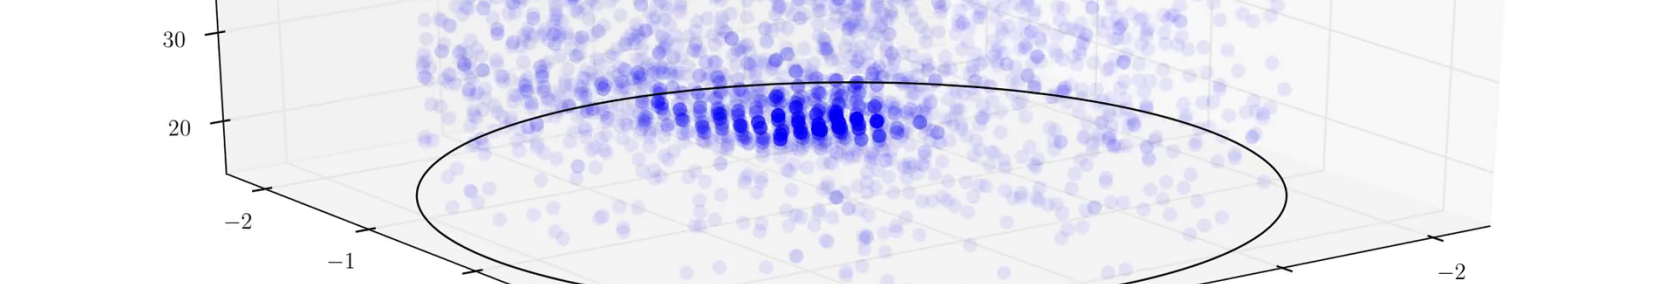
\includegraphics[width=0.8\linewidth]{fig/title.png}}

% Datum:
\date{20. March 2018}
\date[20. March 2018]{DPG-Frühjahrstagung 2018 Würzburg}
% Lehrstuhl/Fakultät:
\institute[TU Dortmund]{Lehrstuhl für Experimentelle Physik 5}

\institute[%
  {
\includegraphics[height=\headerheight]{logos/fact.pdf}}%
  \hspace{1em}%
  {
\includegraphics[height=\headerheight]{logos/e5logo.pdf}}%
]{
  {
\includegraphics[height=0.75cm]{logos/tu.pdf}}%
  \hspace{1em}%
  {
\includegraphics[height=0.75cm]{logos/ethz.pdf}}%
  \hspace{1em}%
  {
\includegraphics[height=0.75cm]{logos/isdc.pdf}}%
  \hspace{1em}%
  {
\includegraphics[height=0.75cm]{logos/uniwue.pdf}}%
}

% Titelgrafik:
% \titlegraphic{
\includegraphics[width=0.4\textwidth]{logos/FACTLogo_preliminary.png}\hfill
\includegraphics[width=0.4\textwidth]{logos/e5logo_green_text.pdf}}
